\chapter{Theoretical aspects}
\label{cha:theorethicalAspects}

In this chapter I would like to describe theory standing behind my work and how is it used nowadays.

%---------------------------------------------------------------------------

\section{State of the Art}
\label{sec:stateOfTheArt}

Nowadays broadly understood data becomes one of the most desired needed resource, everyone wants to make research about everything. For example a lot of mobile applications wants its user to let it access localization or allow it to send some information to servers. But more data we have, the more time it requires from human to process it and extract only things we need. Top it all off it needs to be interpreted afterwards to make some sense of it. That is why Data Science becomes so popular these days. It tries to solve the problem of growing time taken to process bigger and bigger sets of data. The solution turned out to be simple - "let the machines do the work". That is how Machine Learning (ML) was born. Computer Vision (CV) in the other hand is an Artificial Intelligence (AI) branch specified for working with image/video and it uses ML algorithms as a step to achieve its goals of extracting needed data from images/videos with as little human work as possible. As of today CV finds more and more application in various science branches. The most known use of CV is development of Autonomous Driving. There is also technology for monitoring and prevention of pests and grass diseases\cite{appResearch}, based on CV. Also as a example, China's government works on spread of street cameras with face recognition software, but that is less of a positive example as some would say, used for human behaviour control. But in my knowledge there is no Visual Bicycle Counter in commercial application.


%---------------------------------------------------------------------------

\section{What a Bicycle Counter is and why make it "Visual"}
\label{sec:why}

Bicycle Counter, as the name suggest is a device for counting cyclists driving by specific street or bike path. Usually it is a convection loop embedded in asphalt of a road, but photocells installed by the roadside are getting more popular too. Both devices count cyclists passing by and save the number on some sort of server, to make it accessible to obtain for authorized people. Those information can later serve as a good indicator of bicycle traffic in the city. In figure \ref{fig:countersKrakow} we can see that in Krakow there is 17 of those devices installed in across the city and numbers from them are publicly available.
\begin{figure}[H]
    \centering
    \resizebox{\textwidth}{!}{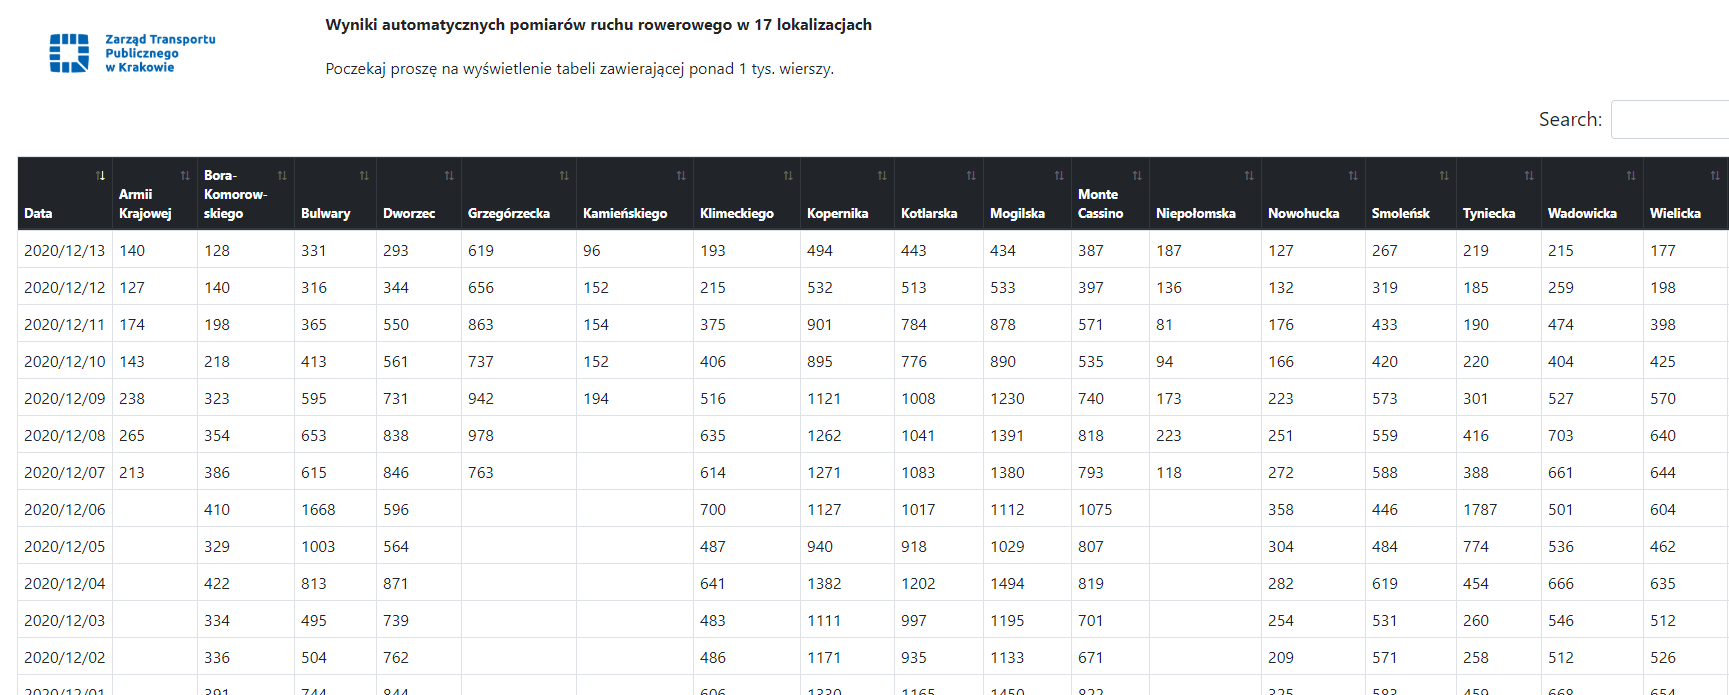
\includegraphics{images/countersKrakow}}
    \caption{First rows of data from bicycle counters installed in Krakow \cite{mobilnykrakow}}
    \label{fig:countersKrakow}
\end{figure}
But why even bother about making Visual Bicycle Counter? First of all, devices I mentioned above are all another equipment used with only one purpose - counting cyclists, so their reusability leaves a lot to be desired. Secondly, installing such a device requires to put more work into it, because you need to for example make a hole in road, put a convection loop in and patch the hole up. Same as maintenance can be problematic too. Visual Bicycle Counter could solve those issues. It uses trained ML model to perform inference on video files from street cameras downloaded on computer or straight on video streams from websites which share it publicly. That would not add next device, but would use existing infrastructure of street cameras, widely developed in many cities.


%---------------------------------------------------------------------------

\section{Short theory behind Visual Bicycle Counter}
\label{sec:theory}

Visual Bicycle Counter bases on deep learning model, what has advantage over traditional target detection. "The traditional method is to manually extract features and require experts in related fields to manually design and process them through years of accumulation and experience. The method of deep learning can learn the features of difference in response data through a large amount of data and is more representative. The deep learning model simulates the human brain's visual perception system. It extracts features directly from the original image, and the features are passed through the layer by layer to obtain the high-dimensional information of the image, making it a great success in the field of computer vision."\cite{deepLearning} But first I had to train my model what consists of collecting data to create a dataset for training (in my case: label video frames - show exactly where cyclist is, divide labelled frames to train and test). Training the model is "showing" computer training data, it learns those and based on what is learns it tries to predict desired information on test data and then process is repeated many, many times until reaching satisfactory parameters. For me, main metrics were: Loss, Recall, Precision. Loss is basically a target function, that is minimized in optimization process (the lower the better and it gets lower when model predicts more accurately). Recall means how many items that should be selected was actually selected, and Precision means how many selected items are actually our desired items. Visualization of Recall and Precision is shown in figure \ref{fig:RPL}.

\begin{figure}[H]
    \centering
    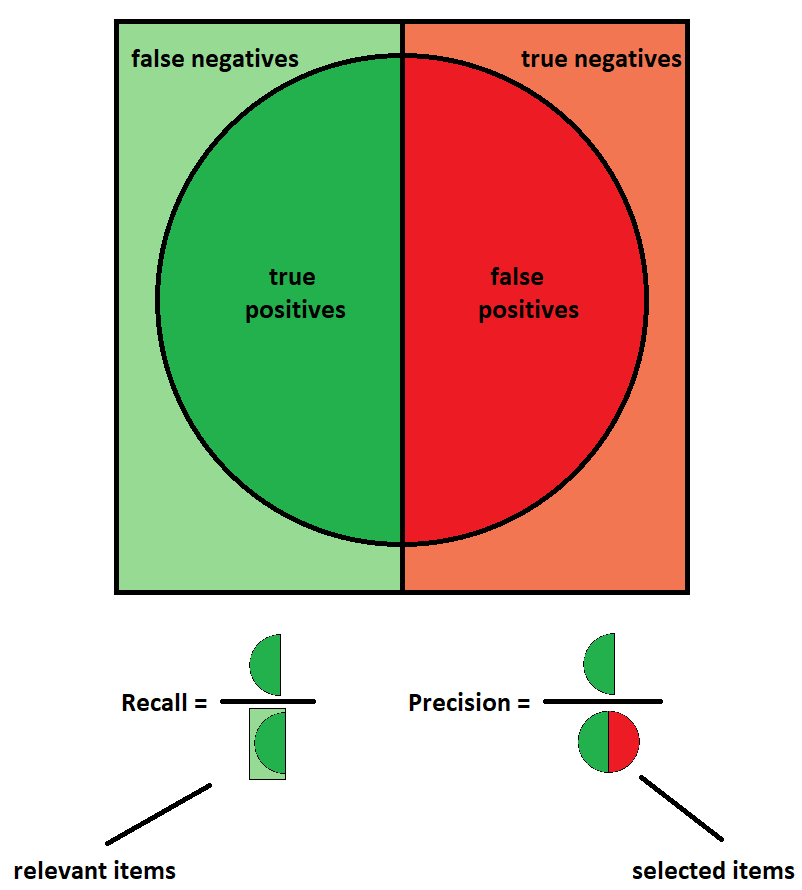
\includegraphics[scale=0.5]{images/rpl}
    \caption{Recall and Precision}
    \label{fig:RPL}
\end{figure}


%---------------------------------------------------------------------------
\section{Tools selection}
\label{sec:tools}

Tools I have used to create my Visual Bicycle Counter were as follow:
\begin{itemize}
    \item youtube-dl software for downloading video streams from street cameras as mp4 files
    \item Virtual Machine with Ubuntu 18.04.5 LTS for download scheduling 
    \item Google Colaboratory as working environment,
    \item Python programming language,
    \item OpenCV libraries for object detection (used by YOLOv5 API),
    \item YOLOv5 API for training YOLO\cite{Redmon_2016_CVPR} models and performing inference,
    \item Wandb for training evaluation.
\end{itemize}
Most of the choices was pretty obvious. I was looking for widely used solutions that provides good documentation and big user base. Youtube-dl was the easiest tool to install and use. Using Google Colaboratory (GC) machine was not only my choice, but at certain stage of work I simply needed more powerful GPU and CPU. GC provided all that as well as Python programming language support. Biggest challenge appeared when I was looking for Object Detection tools. I had to test different solutions, as Tensorflow with Keras, but I found it to be not suitable for my use case so I decided to use OpenCV libraries, YOlOv5 API and Wandb that appeared much more user friendly and provided all features I needed.
